\let\negmedspace\undefined
\let\negthickspace\undefined
\documentclass[journal,12pt,twocolumn]{IEEEtran}
\usepackage{cite}
\usepackage{amsmath,amssymb,amsfonts,amsthm}
\usepackage{algorithmic}
\usepackage{graphicx}
\usepackage{textcomp}
\usepackage{xcolor}
\usepackage{txfonts}
\usepackage{listings}
\usepackage{enumitem}
\usepackage{mathtools}
\usepackage{gensymb}
\usepackage{comment}
\usepackage[breaklinks=true]{hyperref}
\usepackage{tkz-euclide} 
\usepackage{listings}                                   
\def\inputGnumericTable{}                                 
\usepackage[latin1]{inputenc}                                
\usepackage{color}                                            
\usepackage{array}                                            
\usepackage{longtable}                                       
\usepackage{calc}                                             
\usepackage{multirow}                                         
\usepackage{hhline}                                           
\usepackage{ifthen}                                           
\usepackage{lscape}
\newtheorem{theorem}{Theorem}[section]
\newtheorem{problem}{Problem}
\newtheorem{proposition}{Proposition}[section]
\newtheorem{lemma}{Lemma}[section]
\newtheorem{corollary}[theorem]{Corollary}
\newtheorem{example}{Example}[section]
\newtheorem{definition}[problem]{Definition}
\newcommand{\BEQA}{\begin{eqnarray}}
\newcommand{\EEQA}{\end{eqnarray}}
\newcommand{\define}{\stackrel{\triangle}{=}}
\newcommand{\brak}[1]{\langle #1 \rangle}
\theoremstyle{remark}
\newtheorem{rem}{Remark}

\begin{document}
\bibliographystyle{IEEEtran}
\vspace{3cm}
\title{\textbf{GATE 2023 EC}}
\author{EE23BTECH11023-ABHIGNYA GOGULA}
\maketitle
\newpage
\bigskip
\renewcommand{\thefigure}{\theenumi}
\renewcommand{\thetable}{\theenumi}
\textbf{Question28:}
\\
 The Fourier transform $X(\omega)$ of $x(t) = e^{-t^2}$ is\\
Note:$\int_{-\infty}^{\infty} e^{-y^2} \,dy = \sqrt{\pi}$ \\  
A) $\sqrt{\pi} e^{\frac{\omega^2}{2}}$ \\
B) $\frac{e^{\frac{-\omega^2}{4}}}{2\sqrt{\pi}}$ \\
C) $\sqrt{\pi} e^{\frac{-\omega^2}{4}}$ \\
D) $\sqrt{\pi} e^{\frac{-\omega^2}{2}}$\\
\hfill Gate 2023 EC Question 28\\
\textbf{Solution}
\begin{align}
x^{'}(t)=-2te^{-t^{2}}\\
x^{'}(t)=-2tx(t)
\end{align}
doing fourier transform 
\begin{align}
j 2 \pi f X(f)= -2j\frac{d X(f)}{df}\\
\int_{0}^{f} \frac{d X(f)}{X(f)}=\int_{0}^{f} \frac{2 \pi f df}{-2}\\
\frac{X(f)}{X(0)}=e^{\frac{-\brak {2 \pi f}^{2}}{4}}\\
X(0)=\int_{-\infty}^{\infty} x(t)\,dt = \sqrt{\pi}\\
X(f)=\sqrt{\pi}e^{\frac{-\brak {2 \pi f}^2}{4}}\\
X(f)=\sqrt{\pi}e^{-\brak{\pi f}^2}
\end{align}
\begin{figure}[h]
    \centering
    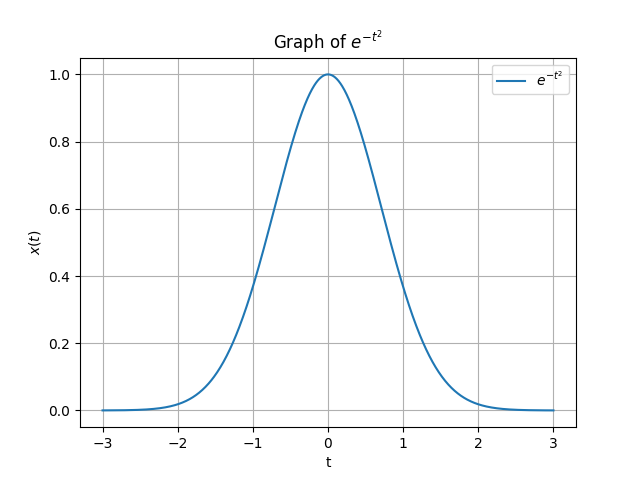
\includegraphics[width=0.5\textwidth]{graph.png}
    \caption{Graph of $e^{-t^2}$}
    \label{fig:plot}
\end{figure}
\begin{figure}[h]
    \centering
    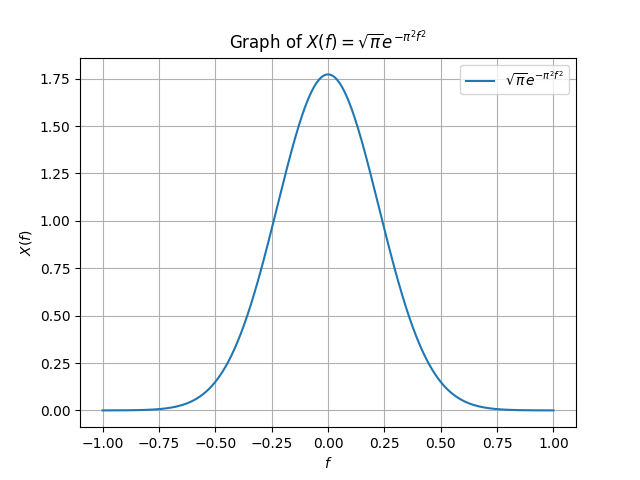
\includegraphics[width=0.5\textwidth]{graph1.png}
    \caption{Graph of $X(f) = \sqrt{\pi}e^{-\pi^2f^2}$}
    \label{fig:plot}
\end{figure}
\end{document}
